%Introduction to state charts
\section{Overview of State Machines} \label{sec:overviewstatechart}

Our proposed visual programming language is modeled by state machines with guarded edges. The language to describe the state machines differs in a few areas from the  \emphasize{UML2 State Machine Diagram}\cite{UML2} syntax in order to support features of the hardware. To better understand these differences we will first introduce the syntax and semantics of more traditional \emphasize{Finite State Machines}\cite{booth} and \emphasize{UML2 State Machine Diagrams}\cite{UML2}.

\begin{definition}
A \emphasize{Finite State Machine} is defined as $M = \lbrace Q, I, Z, \delta, \omega, q_0\rbrace$

\label{def:statecharts}
\begin{itemize}
	\item $Q$: Set of states.
	\item $I$: Set of input symbols.
	\item $Z$: Set of output symbols.
	\item $\delta$: A state transition function: $I \times Q \rightarrow Q$. 
	\item $\omega$: An output function: $Q \rightarrow Z$
	\item $q_0$: Starting state.
\end{itemize}
\end{definition}

A state represents an operating condition. For example in Figure \ref{fig:state_blink_light} the states are ``Light On'' and ``Light Off''.

\begin{figure}[htp]
    \centering
    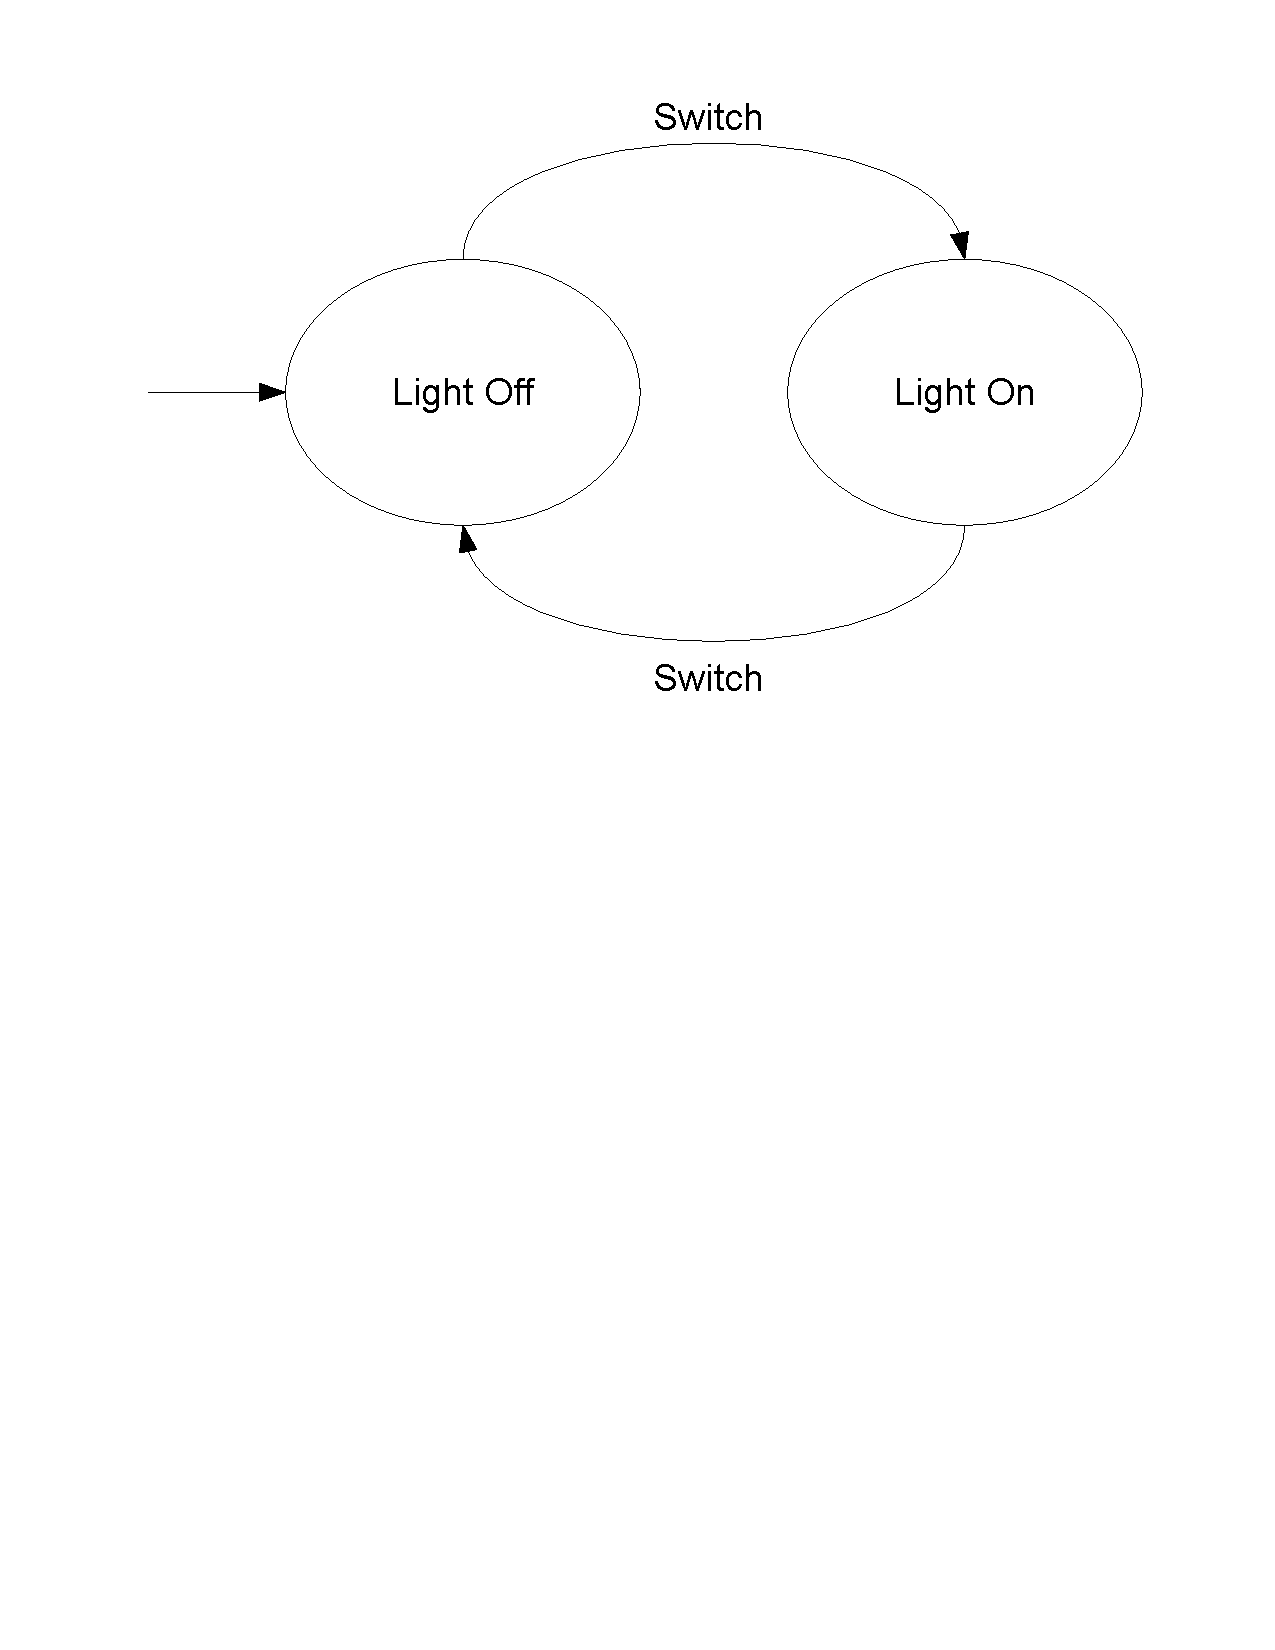
\includegraphics[trim= 10mm 150mm 10mm 10mm, clip, width=\imgmedium]{./images/state_blink_light.pdf}
    \caption{Simple Toggle Light}
    \label{fig:state_blink_light}
\end{figure}

Given a state $q_1 \in Q$ an input $i \in I$ a transition is then a function $\delta(i,q_1) = q_2$ where $q_2$ is the next state and $q_2 \in Q$.  Outputs are formalized to $\omega(q_1)=z_1$ where $z_1 \in Z$. Machines that satisfy Definition \ref{def:statecharts} are referred to as \emphasize{Moore machines}\cite{booth}. A \emphasize{Mealy machine} is obtained by adjusting outputs to be dependent on inputs as well as states. To obtain a \emphasize{Mealy machine} from Definition \ref{def:statecharts} we change our output function to $I \times Q \rightarrow Z$. Although Figure \ref{fig:state_moore_mealy} contains outputs for all edges, we can define a null or a no change output in order to simulate an edge having no output as well. For purposes of the \plccharts language we do not require the power of a Mealy machine and thus we chose to keep our definitions closer to a Moore machine. More details of this decision can be found in Section \ref{sec:statechartsem}.

%diagram for Moore + Mealy state machines
\begin{figure}[htp]
    \centering
    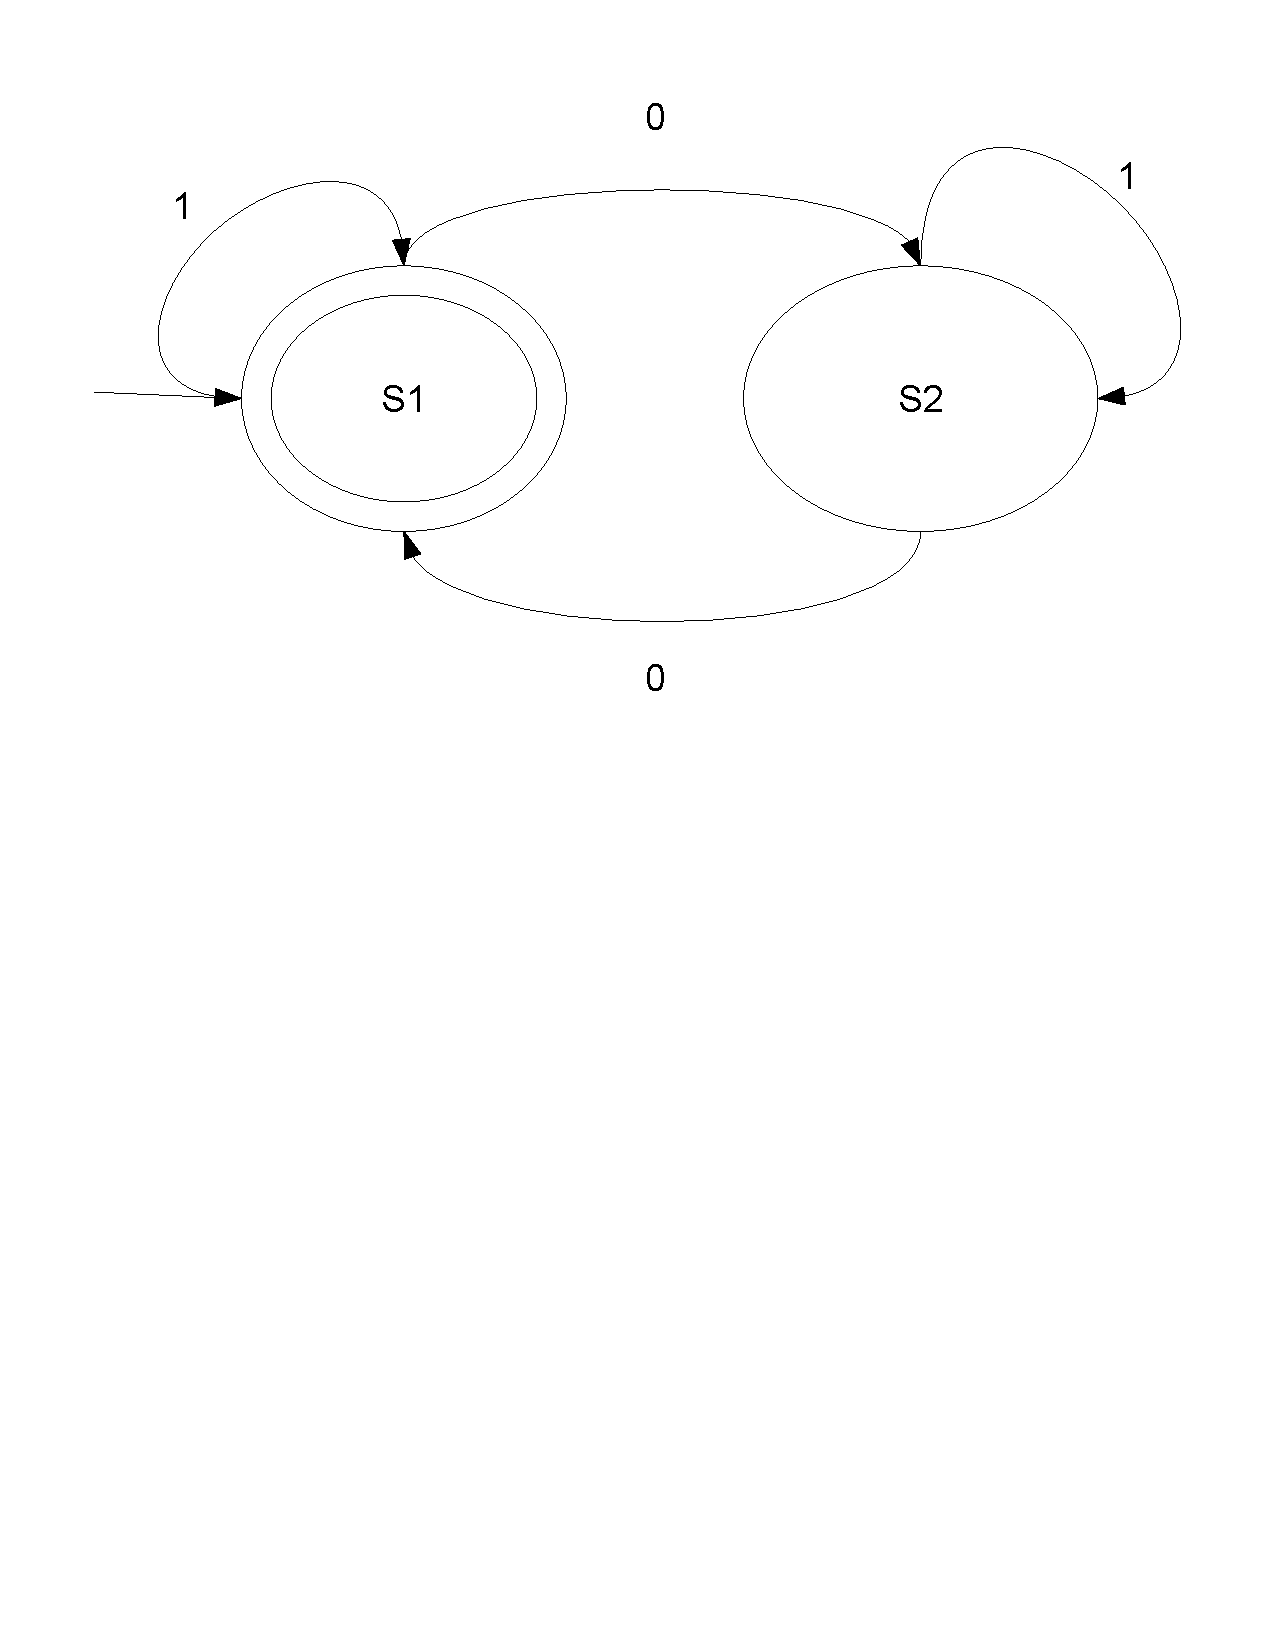
\includegraphics[trim= 15mm 150mm 15mm 10mm, clip, width=200pt]{./images/state_moore.pdf} 
    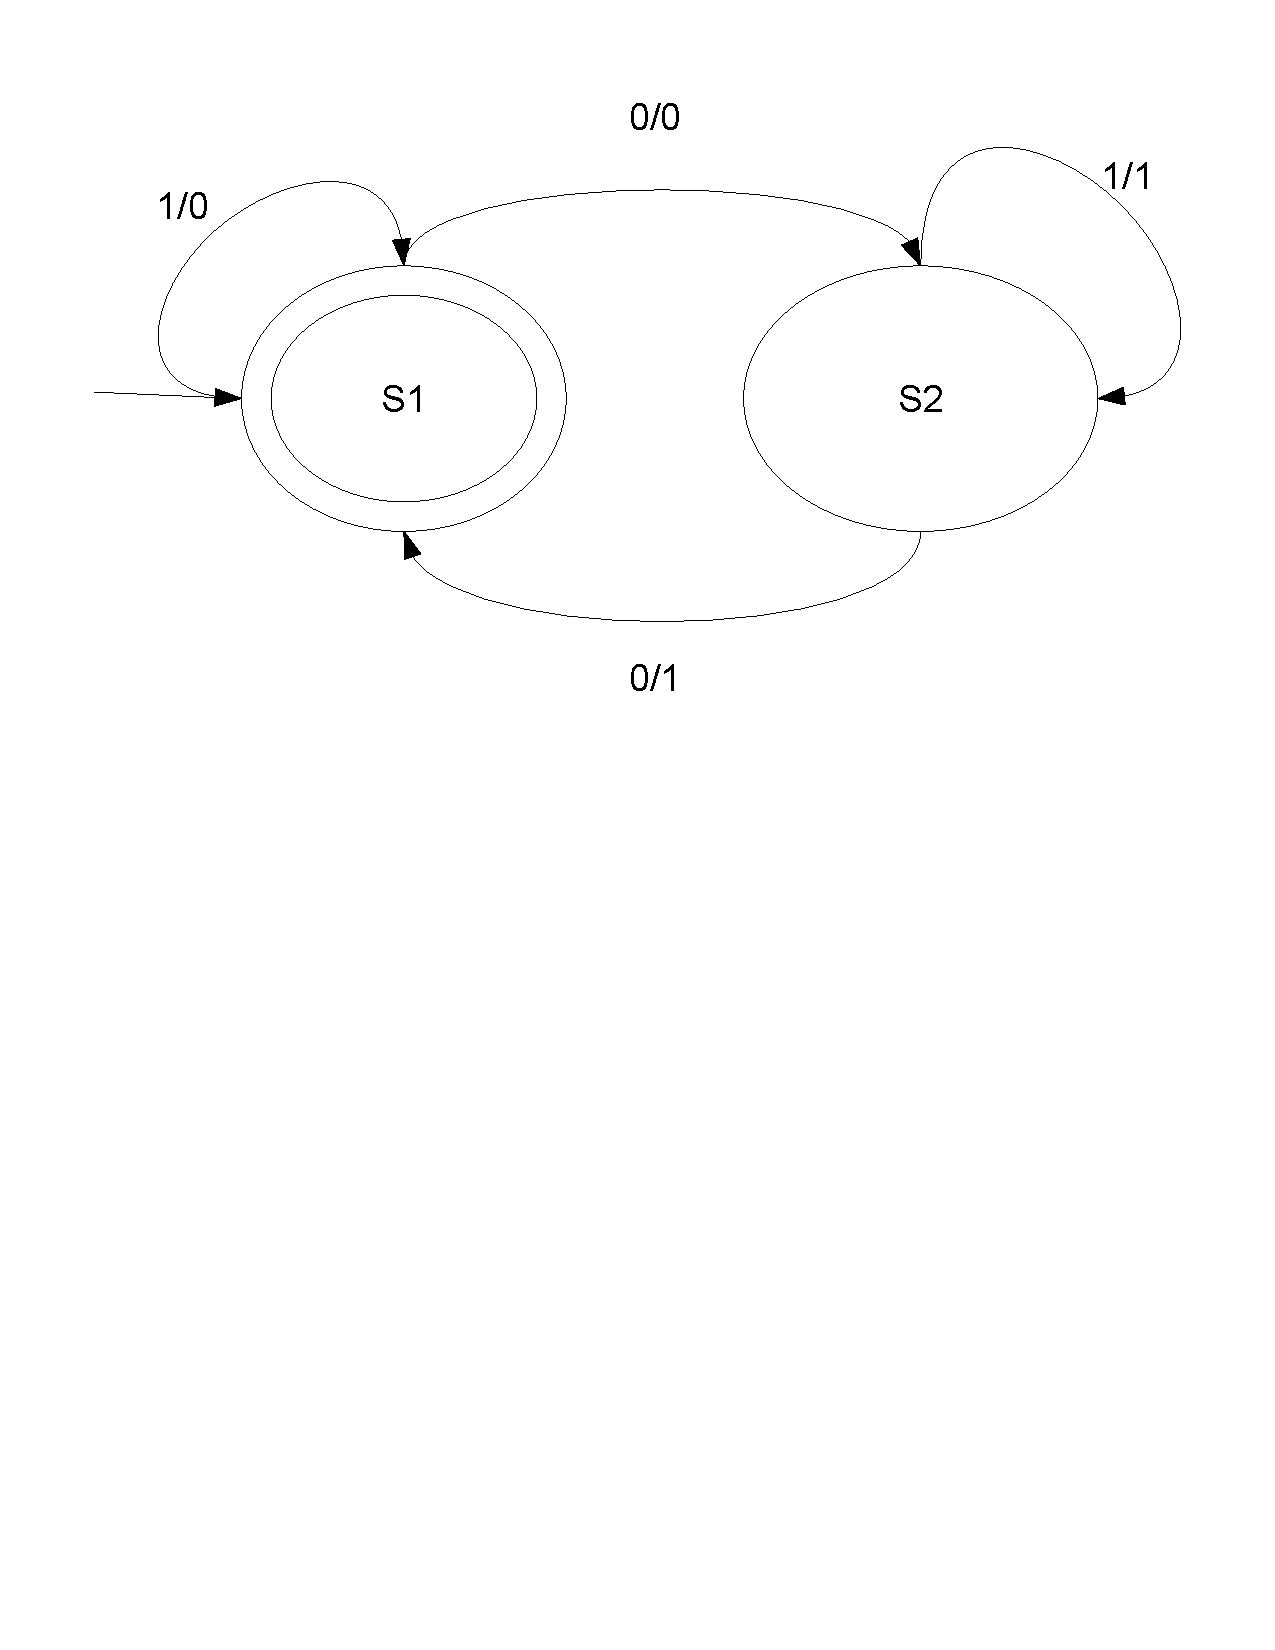
\includegraphics[trim= 15mm 150mm 15mm 10mm, clip, width=200pt]{./images/state_mealy.pdf}    
    \caption{Moore (left) and Mealy (right) State Machines}
    \label{fig:state_moore_mealy}
\end{figure}

To describe our state machines we use diagrams such as adopted by \emphasize{UML}\cite{UML2}. There are several ways a starting state can be drawn as seen in Figure \ref{fig:state_moore_mealy}.
One such way is to draw a edge that has no state connected to its tail. In our system we choose incorporate a symbol similar to  the \emphasize{UML}\cite{UML2} symbol where the start state edge has a solid dot connected to the tail as shown in Figure \ref{fig:state_uml_light}. {\plccharts} utilizes a special \emphasize{start} state that is functionaly identical to \emphasize{UML's} solid dot symbol.

%diagram for UML state machines
\begin{figure}[htp]
    \centering
    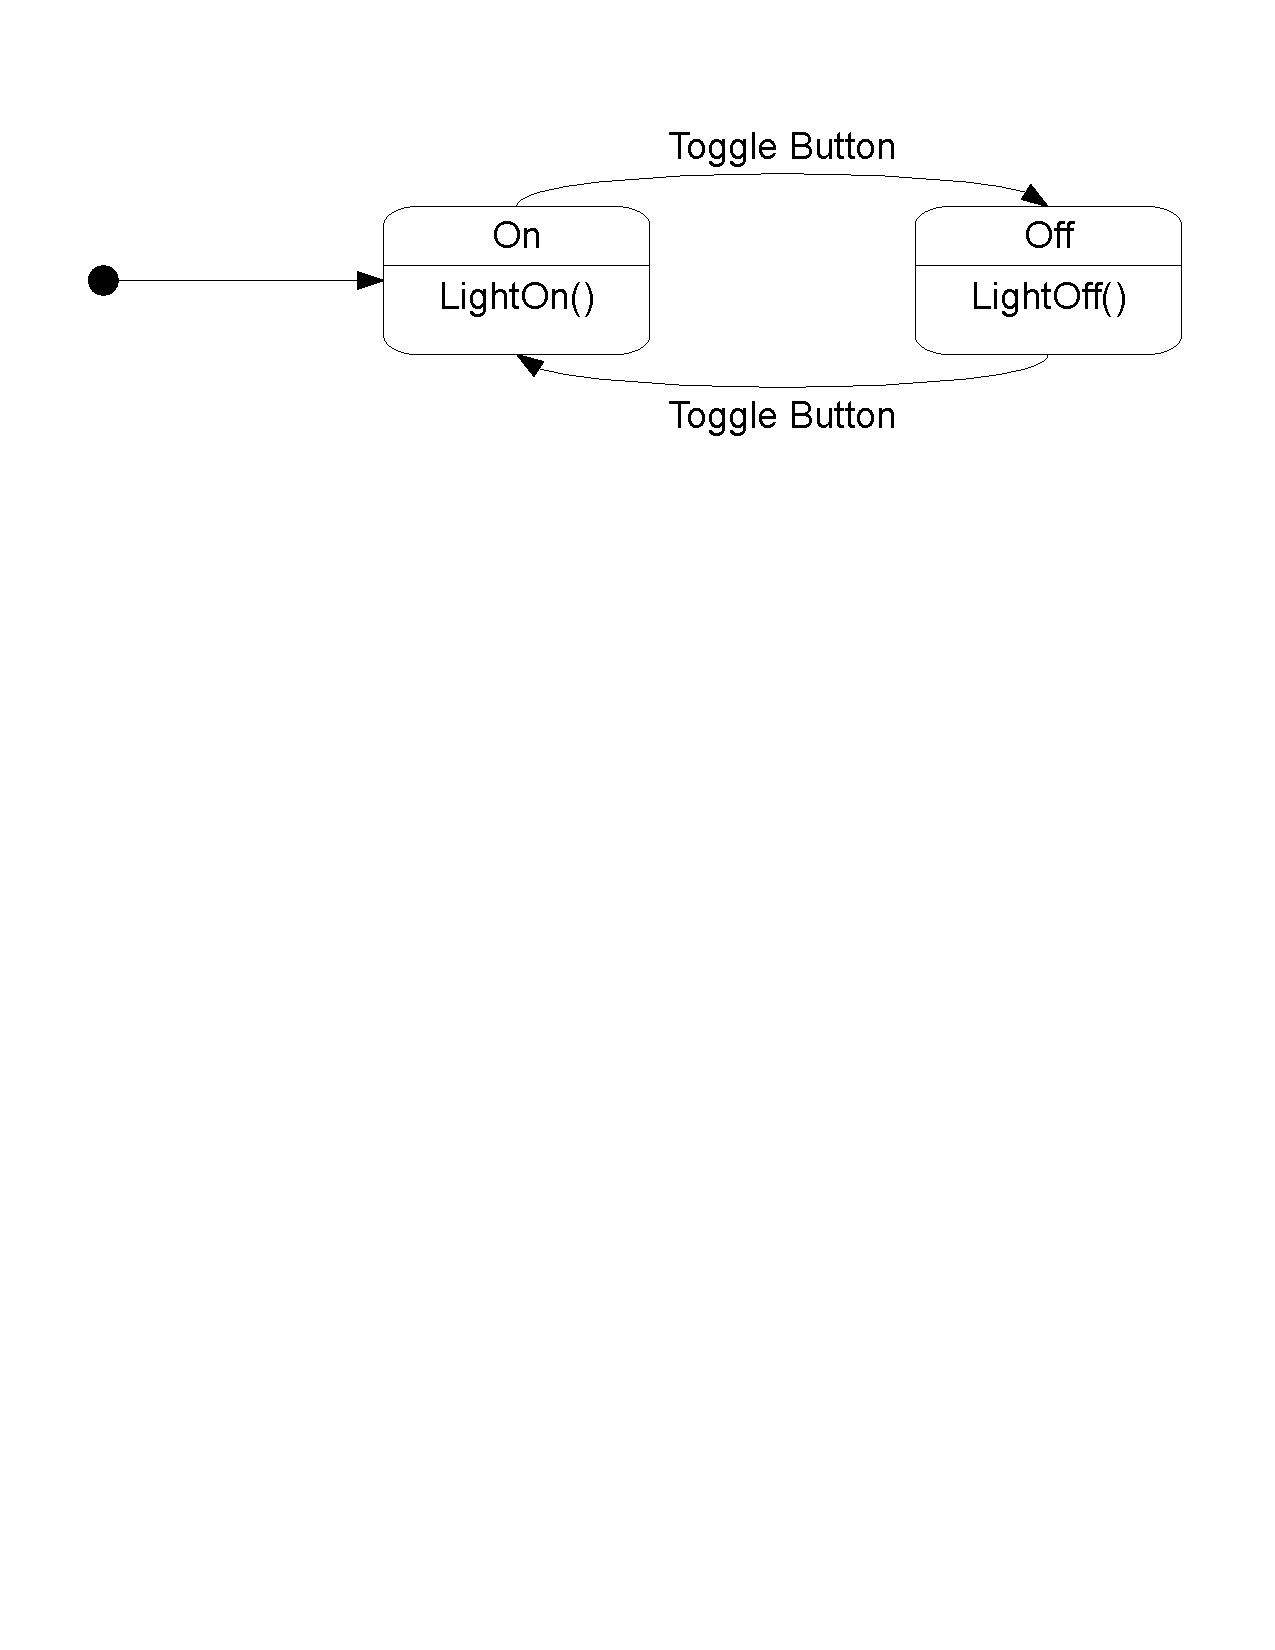
\includegraphics[trim= 15mm 200mm 15mm 10mm, clip, width=\imgmedium]{./images/state_uml_light.pdf} 
    \caption{UML State Diagram of a Toggle Light}
    \label{fig:state_uml_light}
\end{figure}

The \emphasize{UML State Diagram}\cite{UML2} as shown in Figure \ref{fig:state_uml_light} also allows for state titles in each state seen at the top of each state. In addition, each state may contain actions that are executed. In Figure \ref{fig:state_uml_light} ``LightOn()'' and ``LightOff()'' refer to executed actions that are called once the ``On'' and ``Off'' states are reached. The behaviour is read as once the state ``On'' is reached ``LightOn()'' is executed right away. More than one instruction to be executed can be listed and is understood that each instruction is executed sequentially\cite{UML2}.

\clearpage
%diagram for UML state machines
\begin{figure}[htp]
    \centering
    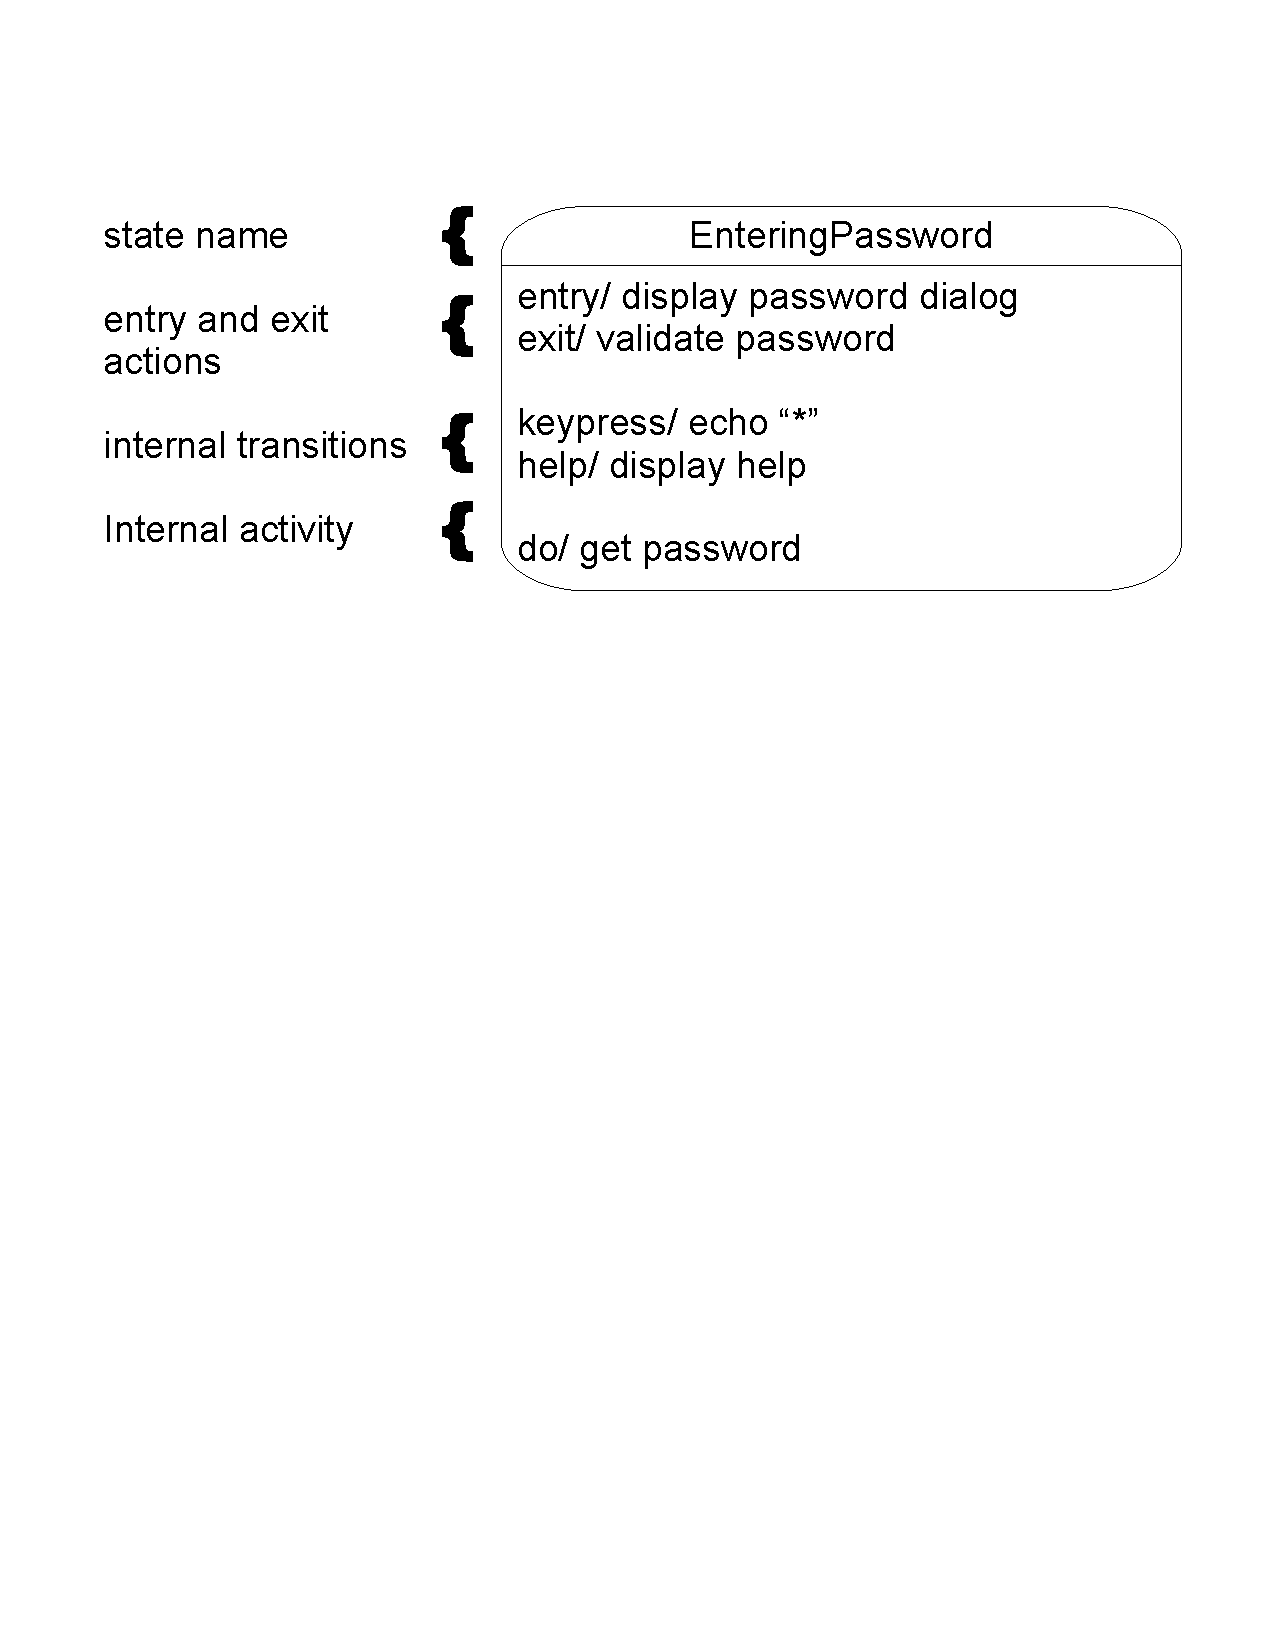
\includegraphics[trim= 15mm 175mm 15mm 10mm, clip, width=\imgmedium]{./images/state_uml2_syntax_21_4.pdf} 
    \caption{UML2 State Machine Diagram Syntax\cite{UML2}}
    \label{fig:state_uml2}
\end{figure}

The syntax shown in Figure \ref{fig:state_uml_light} is that of \emphasize{UML2 State Machine Diagram}\cite{UML2}. Each state bubble in  \emphasize{UML2 State Machine Diagram} contains the information given by Definition \ref{def:uml2} and shown in Figure \ref{fig:state_uml2}. The additional information makes UML2 more useful for representing programs more conveniently.

\begin{definition}
UML2 State Machine Diagram by convention is given by the following:

\label{def:uml2}
\begin{itemize}
	\item \textbf{state name:} The state name is mandatory for each UML2 state in cases where this is the only information the horizontal divider may be omitted.
	\item \textbf{entry and exit actions:} Entry and exit actions are optional, they are commonly used for initializers and finalizers that may occur in each state.
	\item \textbf{internal transitions:} These optional fields refer to simple transitions that may happen in the state itself generally these are simple enough to not require a separate diagram.
	\item \textbf{internal activity:} These are optional and refer to activities that occur or are executed while in the state.
\end{itemize}
\end{definition}
